\documentclass[../INDE315.tex]{subfiles} 
\usepackage{fancyhdr}
\usepackage{graphicx}
\usepackage{amsmath}
\usepackage{mhchem}
\usepackage{amssymb}
\usepackage[margin=1in]{geometry}

\graphicspath{{./images/}}

\title{UW IND E 315 Notes}
\author{Anthony Le}

\begin{document}

\pagestyle{fancy}
\fancyhead{}
\fancyhead[R]{UW IND E 315}
\fancyhead[L]{Anthony Le}

\fancyhead[C]{Chapter 3 - Discrete Random Variables}

\section*{Chapter 3 - Discrete Random Variables}
Continuing from chapter 2, should we always count possible outcomes to calculate probabilities?
\begin{enumerate}
    \item Thankfully no, but it is important to know the counting techniques to understand the fundamentals of probability.
    \item In this chapter, we'll introduce the concept of the \emph{random variable} and a handful of widely used probability distributions which empower engineers to do much more faster.
\end{enumerate}
\subsection*{Random Variables (2.9)}

\begin{defn}
    \textbf{Random Variables} \\
    A random variable is a \emph{function} that assigns \emph{a real number} to each outcome in the sample space of a random experiment. 
    \begin{enumerate}
        \item Denoted by an uppercase letter (ex: $X$)
        \item Its realization is denoted by a lowercase letter (ex: $x$)
    \end{enumerate}
\end{defn}
\begin{exmp}
    $X = 0$ if tails and $X = 1$ if heads.
    \begin{enumerate}
        \item $P(X = x)$ for $x = 0$?
    \end{enumerate}
\end{exmp}

\subsubsection*{Continuous and Discrete Random Variables (rv)}
\begin{defn}
    \textbf{\emph{Discrete} Random Variable} \\
    A random variable (rv) with a \emph{countable} range. 
    \begin{enumerate}
        \item Such as counts, integers, or natural numbers
    \end{enumerate}
\end{defn}

\begin{defn}
    \textbf{\emph{Continuous} Random Variable} \\
    A random variable with an \emph{uncountable range} (usually an interval)
    \begin{enumerate}
        \item Such as length, weight, volume
    \end{enumerate}
\end{defn}

\subsection*{Probability Distributions and Probability Mass Functions (3.1)}

\subsubsection*{Probability Distribution (3.1)}
\begin{defn}
    \textbf{Probability Distribution} \\
    The probability distribution of a random variable $X$ is a description of the probabilities associated with the possible values of $X$. \\
    There are two types of probability distribution:
    \begin{enumerate}
        \item Discrete Probability Distributions (Covered in this chapter)
        \item Continuous Probability Distributions (Covered in chapter 4)
    \end{enumerate}
\end{defn}

\subsubsection*{Probability Mass Function (3.1)}
\begin{defn}
    \textbf{Probability Mass Function} \\
    For a \emph{discrete} random variable $X$ with possible values $x_1, x_2, ...x_n$, a \textbf{probability mass function (PMF)} is a function such that:\footnote{Note - the PMF of X fully characterizes the probability distribution of X.}
    \begin{enumerate}
        \item $f(x_i) \geq 0$
        \item $\sum_{i=1}^{n} f(x_i) = 1$
        \item $f(x_i) = P(X = x_i)$
    \end{enumerate}
\end{defn}
\subsubsection*{Probability Mass Function - Example}
\begin{exmp}
    Let $X$ be the number of days in a year Seattle's highest temperature exceeds 90F.
\end{exmp}

\begin{equation*}
    \begin{aligned}
        f(x) = P(X = x)
    \end{aligned}
\end{equation*}
\begin{center}
    \begin{tabular}{c c c c c c}
        x & 1 & 2 & 3 & 4 & 5 \\
        f(x) & 0.55 & 0.25 & 0.12 & 0.04 & 0.03  
    \end{tabular}        
\end{center}

\begin{equation*}
    \begin{aligned}
        \sum f(x) &= P(X = 1) + P(X = 2) + P(X = 3) + P(X = 4) + P(X = 5) \\
                & = 0.55 + 0.26 + 0.12 + 0.04 + 0.03 \\
                & = 1
    \end{aligned}
\end{equation*} 

\subsubsection*{Cumulative Distribution Function (CDF) (3.2)}
\begin{defn}
    \textbf{Cumulative Distribution Function} \\
    I'm not sure what this is, since the prof doesn't provide the exact definition, but hopefully continuing on the example might help provide a better idea of what it is.
\end{defn}

\begin{center}
    \begin{tabular}{c c c c c c}
        x & 1 & 2 & 3 & 4 & 5 \\
        f(x) & 0.55 & 0.25 & 0.12 & 0.04 & 0.03 \\
        F(x) & 0.55 & 0.81 & 0.93 & 0.97 & 1.00 \\
    \end{tabular}        
\end{center}
Where $F(x)$ is defined as:
\begin{equation*}
    \begin{aligned}
        F(x) &= P(X \leq x) \\
        F(x) &= 
            \begin{cases}
                0 & x < 1 \\
                0.55 & 1 \leq x < 2 \\
                0.81 & 2 \leq x < 3 \\
                0.93 & 3 \leq x < 4 \\
                0.97 & 4 \leq x < 5 \\
                1.00 & x \geq 5
            \end{cases}
    \end{aligned}
\end{equation*}

\subsection*{Mean and Variance of a Discrete Random Variable (3.3)}

\subsubsection*{Mean}
\begin{defn}
    \textbf{Mean or expected value} \\
    The measure of the center of a probability distribution.
\end{defn}

\begin{equation*}
    \begin{aligned}
        \overbrace{\mu}^{\text{mean}} = \underbrace{E(X)}_{\parbox{5cm}{Expected value of the discrete random variable, \emph{X}}} = \sum_{x} x * f(x)       
    \end{aligned}
\end{equation*}

\subsubsection*{Example 3-7}
\begin{exmp}
    X = number of bits in error in the next 4 bits transmitted. \\
    Possible values of X are {0, 1, 2, 3, 4}
    \begin{center}
        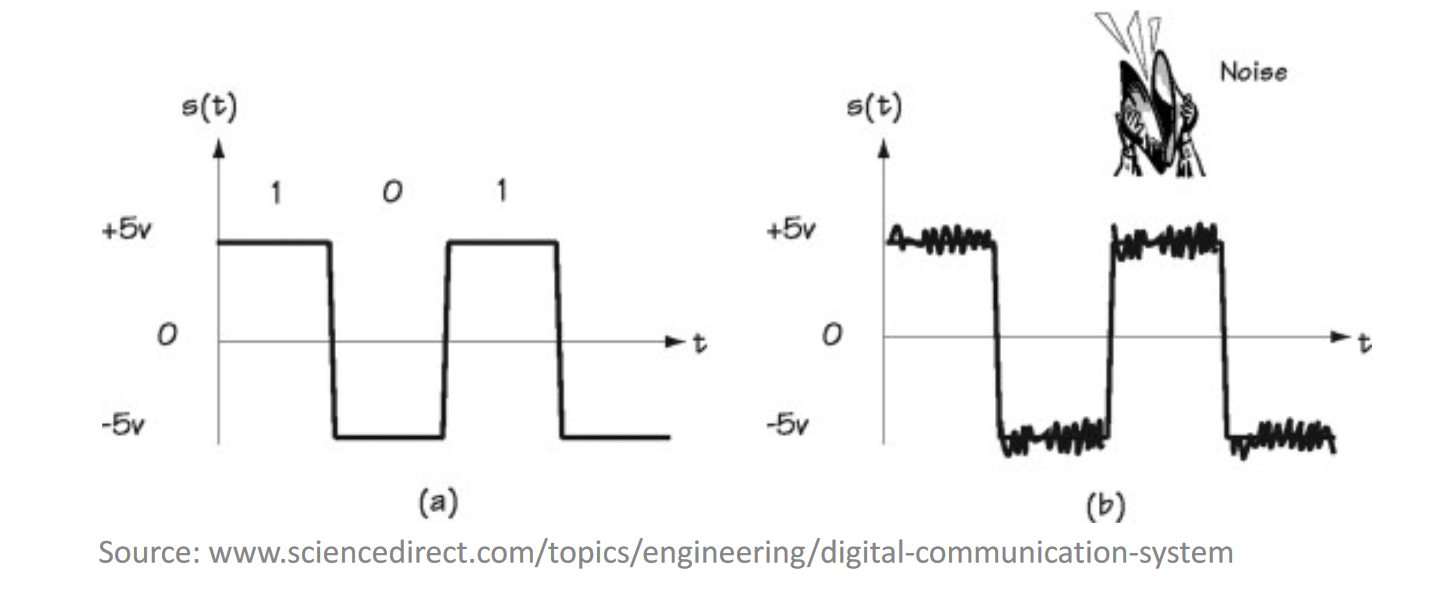
\includegraphics[width = 8cm]{Ch3Example2}
    \end{center}
    Suppose the probabilies will be:
    \begin{equation*}
        \begin{aligned}
            P(X = 0) &= 0.6561 \\
            P(X = 1) &= 0.2916 \\
            P(X = 2) &= 0.0486 \\
            P(X = 3) &= 0.0036 \\
            P(X = 4) &= 0.0001 
        \end{aligned}
    \end{equation*} 
    Find the mean.   
\end{exmp}

\begin{equation*}
    \begin{aligned}
        \mu = E(X) &= \sum_{x} x * f(x) \\
                &= 0 * f(0) + 1 * f(1) + 2 * f(2) + 3 * f(3) + 4 * f(4) \\
                &= 0 * (0.6561) + 1 * (0.2916) + 2* (0.0486) + 3 * (0.0036) + 4 * (0.0001) \\
            \mu &= 0.4 
    \end{aligned}
\end{equation*} 

\subsubsection*{Variance}
\begin{defn}
    \textbf{Variance} \\
    Measure of the dispersion or varability in a probability distribution.
    \begin{equation*}
        \begin{aligned}
            \overbrace{\sigma ^2}^{\text{Variance}} &= V(X) = E(X - \mu)^2 \\
                                                &= \sum_x (x- \mu)^2 * f(x) \\
                                                &= \sum_x x^2 * f(x) - \mu ^2 
        \end{aligned}
    \end{equation*}
    Alternatively, the better method for calculations would be:
    \begin{equation*}
        \begin{aligned}
            \sigma ^2 =  Var(X) = E[X^2] - (E[X])^2 \\
            \\
            E[f(x)] = \sum f(x) p(x) 
        \end{aligned}
    \end{equation*}
\end{defn}

\subsubsection*{Example 3-7 Continued}
% In this section, we're finding the variance after we found the mean.
\begin{exmp}
    X = number of bits in error in the next 4 bits transmitted. \\
    Possible values of X are {0, 1, 2, 3, 4}. \\
    Find the variance.
\end{exmp}
We know from our prior calculation that $\mu = 0.4$, so:
\begin{equation*}
    \begin{aligned}
        \sigma ^2 = V(X) &= E(X - \mu)^2 = \sum_x (x - \mu)^2 * f(x) \\
        \sigma ^2        &= \sum_x (x - 0.4)^2 * f(x)
    \end{aligned}
\end{equation*} 
We now have a general formula for the variance - along with the probabilities we're given, we can make a table to find the individual variance for each x and sum them up to find the total variance:
\begin{enumerate}
    \item Given numbers:
        \begin{center}
            \begin{tabular}{c c}
                $x$ & $f(x)$ \\
                \hline \\
                0 & 0.6561 \\
                1 & 0.2916 \\
                2 & 0.0486 \\
                3 & 0.0036 \\
                4 & 0.0001 
            \end{tabular}
        \end{center}
    \item Adding in helper columns
        \begin{center}
            \begin{tabular}{c c c c c}
                $x$ & $x-0.4$ & $(x-0.4)^2$ & $f(x)$ & $f(x) (x-0.4)^2$\\
                \hline \\
                0 & & & 0.6561 & \\
                1 & & & 0.2916 & \\
                2 & & & 0.0486 & \\
                3 & & & 0.0036 & \\
                4 & & & 0.0001 &
            \end{tabular}
        \end{center}
    \item Solving for values
        \begin{center}
            \begin{tabular}{c c c c c}
                $x$ & $x-0.4$ & $(x-0.4)^2$ & $f(x)$ & $f(x) (x-0.4)^2$\\
                \hline \\
                0 & -0.4 & 0.16 & 0.6561 & 0.104976     \\
                1 & 0.6 & 0.36 & 0.2916 &  0.104976     \\
                2 & 1.6 & 2.56 & 0.0486 &  0.124416     \\
                3 & 2.6 & 6.76 & 0.0036 &  0.024336     \\
                4 & 3.6 & 12.96 & 0.0001 & 0.001296     \\
                \hline
                    & & & & 0.360000
            \end{tabular}
        \end{center}
    \item Summing altogether
        \begin{equation*}
            \begin{aligned}
                \sigma ^2 = V(X) &= E(X - \mu)^2 = \sum_x (x - \mu)^2 * f(x) \\
                            &= 0.360000
            \end{aligned}
        \end{equation*}
\end{enumerate}

\subsubsection*{Standard deviation}
\begin{defn}
    \textbf{Standard deviation} \\
    Another measure of the dispersion. It is the square root of the variance.
    \begin{equation*}
        \begin{aligned}
            \sigma = \sqrt{\sigma ^2}
        \end{aligned}
    \end{equation*}
\end{defn}
\begin{exmp}
    Using example 3-7, find the standard deviation.
\end{exmp}
\begin{equation*}
    \begin{aligned}
        \sigma ^2 &= 0.360000 \\
        \sigma &= \sqrt{0.360000} \\
        \sigma &= 0.6
    \end{aligned}
\end{equation*}

\subsubsection*{Some other properties to note}
\begin{enumerate}
    \item $E(aX) = aE(X)$
    \item $E(aX + b) = aE(X) + b$
    \item $E[f(X)] = \sum f(x) p(x)$
    \item $V(aX) = a^2 V(X)$
    \item $V(aX + B) = a^2 V(X)$
\end{enumerate}

\subsection*{Discrete Uniform Distribution (3.4)}
\begin{defn}
    \textbf{Discrete Unifrom Distribution} \\
    Definitions:
    \begin{enumerate}
        \item A random variable $X$ has a discrete uniform distribution if each of the $n$ values in its range, say $x_1, x_2, ... x_n$ has an \emph{equal} probability of occurring.
            \begin{equation*}
                \begin{aligned}
                    f(x_i) = \frac{1}{n}
                \end{aligned}
            \end{equation*} 
        \item Alternatively, let $X$ be a discrete uniform random variable with the range of consecutive integers $a, a+1,...,b$ for $a \leq b$. Then for any $x$ in the range,
            \begin{equation*}
                \begin{aligned}
                    f(x) = \frac{1}{b - a + 1}
                \end{aligned}
            \end{equation*}
    \end{enumerate}
\end{defn}

\subsubsection*{Discrete Uniform Distribution Example - Dice}
For rolling a fair dice, using a cumulative distribution function (CDF): \\
Givens:
\begin{enumerate}
    \item S = {1, 2, 3, 4, 5, 6}
    \item Probabilities:
        \begin{equation*}
            \begin{aligned}
                F(x_i) = P(X \leq 1) &= 1/6 \\
                P(X \leq 2) &= 2/6  \\
                P(X \leq 3) &= 3/6 \\
                P(X \leq 4) &= 4/6 \\
                P(X \leq 5) &= 5/6 \\
                P(X \leq 6) &= 6/6 \\
            \end{aligned}
        \end{equation*}
        \begin{center}
            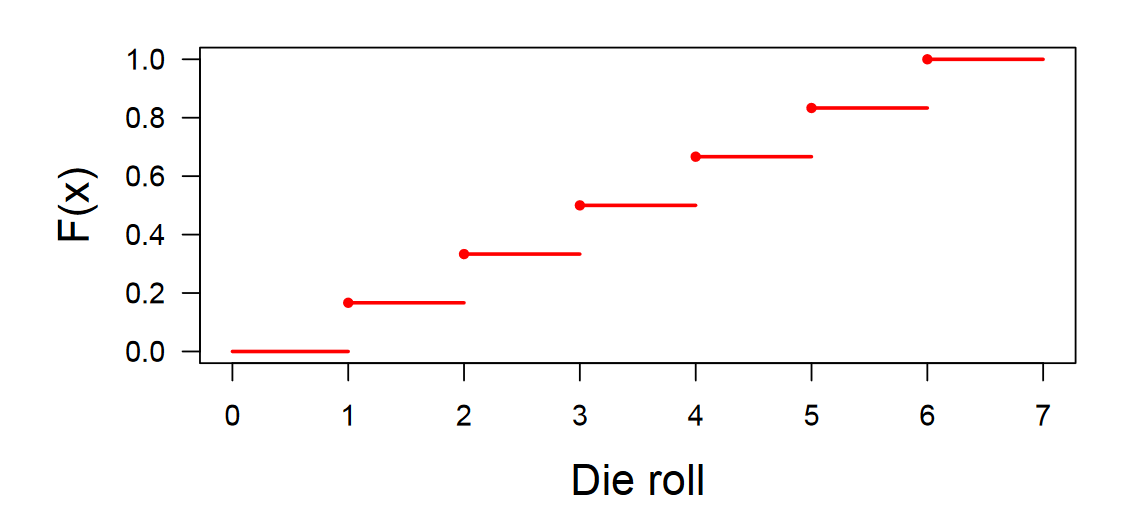
\includegraphics[width = 8cm]{Ch3_UniformDistribution_Discrete}
        \end{center}
\end{enumerate}

\subsubsection*{Mean and Variance for Discrete Uniform Distribution\footnote{using the second definition, where a and b represent the upper and lower bounds for the range of consecutive integers respectively.}}
\begin{enumerate}
    \item Mean:
        \begin{equation*}
            \begin{aligned}
                \mu = E(x) = \frac{b + a}{2}
            \end{aligned}
        \end{equation*}
        Using the die example:
        \begin{equation*}
            \begin{aligned}
                \mu = E(x) &= \frac{6 + 1}{2} \\
                        &= 3.5
            \end{aligned}
        \end{equation*}
    \item Variance:
        \begin{equation*}
            \begin{aligned}
                \sigma ^2 = V(x) = \frac{(b - a + 1)^2 - 1}{12}
            \end{aligned}
        \end{equation*}
        Using the die example:
        \begin{equation*}
            \begin{aligned}
                a ^2 = V(x) &= \frac{(6 - 1 + 1)^2 - 1}{12} \\
                        &= 2.917
            \end{aligned}
        \end{equation*}
\end{enumerate}

\subsection*{Binomial Distribution (3.5)}
\begin{defn}
    \textbf{Bernoulli Trial} \\
    Describes a trial with ONLY two possible outcomes (such as pass/fail, yes/no, 0/1, etc.).
\end{defn}

\begin{defn}
    \textbf{Binomial Distribution} \\
    A distribution based on $n$ Bernoulli Trials such that:
    \begin{enumerate}
        \item The trials are independent;
        \item Each trial results in two possible outcomes, labeled as "success" and "failure"; and
        \item Probability of a success in each trial, $p$, remains constant.
    \end{enumerate}
    To model the number of \textbf{successes} out of $n$ independent trials:\footnote{The excel function for Binomial PMF is BINOM.DIST(x, n, p, FALSE)}
    \begin{equation*}
        \begin{aligned}
            f(x) = \left( \begin{tabular}{c}
                n \\
                x
                \end{tabular}  \right) p^x (1 - p)^{n-x} \quad x = 0, 1, 2, ...,n
        \end{aligned}
    \end{equation*}
    Where:
    \begin{enumerate}
        \item p = probability of success
        \item n = fixed number of independent trials
        \item x = number of \textbf{successes}
        \item n-x = number of \textbf{failures}
    \end{enumerate}
\end{defn}

\subsubsection*{Binomial Distribution Example - coin flips}
\begin{exmp}
    What is the probability of 2 heads in 5 coin flips?
\end{exmp}
\begin{equation*}
    \begin{aligned}
        P(X = 2) = \underbrace{\left( \begin{tabular}{c}
            5 \\
            2
            \end{tabular}  \right)}_{C^5_2} 0.5^2 (1 - 0.5)^{5-2}
    \end{aligned}
\end{equation*}

\begin{exmp}
    What is the probability of AT LEAST 2 heads in 5 coin flips?
\end{exmp}
\begin{equation*}
    \begin{aligned}
        P(X \geq 2) &= 1 - P(X < 2) \\
        P(X \geq 2) &= \sum ^5_{x = 2} \left( \begin{tabular}{c}
            5 \\
            x
            \end{tabular}  \right) 0.5^x (1 - 0.5)^{5-x} \\
        1 - P(X < 2) &= 1 - \sum_{1}^{x=0}\left( \begin{tabular}{c}
            5 \\
            x
            \end{tabular}  \right) 0.5^x (1 - 0.5)^{5-x} \\
    \end{aligned}
\end{equation*}

\subsubsection*{Binomial Mean and Variance}
If $X$ is a binomial random variable with parameters p (probability) and n (number trials), 
\begin{enumerate}
    \item Mean:
        \begin{equation*}
            \begin{aligned}
                \mu = E(X) = np
            \end{aligned}
        \end{equation*}
    \item Variance:
        \begin{equation*}
            \begin{aligned}
                \sigma ^2 = V(X) = np(1-p)
            \end{aligned}
        \end{equation*}
\end{enumerate}

\subsection*{Geometric Distributions (3.6)}
\begin{defn}
    \textbf{Geometric distribution} \\
    A series of Bernoulli trials with fixed parameter $p$. \\
    Binomial distribution has:
    \begin{enumerate}
        \item \textbf{Fixed} number of trials, $n$
        \item \textbf{Random} number of successes, $x$
    \end{enumerate}
    Geometric distribution has:
    \begin{enumerate}
        \item \textbf{Random} number of trials, $x$
        \item \textbf{Fixed} number of successes, \emph{in this case 1}.
        \item i.e. this finds the number of trials until the first success.
    \end{enumerate}
\end{defn}
\subsubsection*{Geometric vs. Binomial Distribution}
Formulas:
\begin{enumerate}
    \item Where $0 \leq p < 1$ and x is the number of trials
    \item Binomial: \footnote{note that for binomial, you need to account for the number of trials}
        \begin{equation*}
            \begin{aligned}
                \text{Probability: } &  f(x) = \left( \begin{tabular}{c}
                    n \\
                    x
                    \end{tabular}  \right) p^x (1 - p)^{n-x} \\
                \text{Mean: } & \mu = E(X) = np \\
                \text{Variance: } & \sigma ^2 = V(X) = np(1-p)
            \end{aligned}
        \end{equation*}
    \item Geometric:
        \begin{equation*}
            \begin{aligned}
                \text{Probability: } &  f(x) = p^1 (1-p)^{x-1} \\
                \text{Mean: } &  \mu = E(X) = \frac{1}{p} \\
                \text{Variance: } & \sigma ^2 = V(X) = \frac{1-p}{p^2}  
            \end{aligned}
        \end{equation*}
\end{enumerate}

\subsubsection*{Example 3-19: Digital Transmission Channel}
\begin{exmp}
    Probability of a bit transmitted in error p = 0.1 \\
    X = number of transmissions until the first error. \\
    Find X from the mean, variance, and standard deviation.
\end{exmp}
\begin{enumerate}
    \item Finding mean:
        \begin{equation*}
            \begin{aligned}
                \mu &= E(X) = \frac{1}{p} = \frac{1}{0.1} \\
                \mu &= 10
            \end{aligned}
        \end{equation*}
    \item Finding variance:
        \begin{equation*}
            \begin{aligned}
                \sigma ^2 &= V(X) = \frac{1-p}{p^2} = \frac{1-0.1}{0.1^2} \\
                \sigma ^2 &= 90
            \end{aligned}
        \end{equation*}
    \item Finding standard deviation:
        \begin{equation*}
            \begin{aligned}
                \sigma &= \sqrt{\sigma ^2} = \sqrt{90} \\
                \sigma &= 9.487
            \end{aligned}
        \end{equation*}
\end{enumerate}

\subsubsection*{Example 3-20: Memoryless Property}
\begin{exmp}
    For the same problem with $p = 0.1$, suppose 50 bits have already been transmitted, what is the mean number of bits transmitted until the next error?
\end{exmp}
\begin{enumerate}
    \item Finding mean:
        \begin{equation*}
            \begin{aligned}
                \mu &= E(X) = \frac{1}{p} = \frac{1}{0.1} \\
                \mu &= 10
            \end{aligned}
        \end{equation*}
\end{enumerate}

\subsection*{Negative Binomial Distribution (3.6)}
\footnote{I guess this is similar to geometric distributions, but now you have the flexibility to do more than just one success.}

\begin{defn}
    \textbf{Negative Binomial Distribution} \\
    $X$ = number of Bernoulli trials required to obtain $r$ successes:
    \begin{equation*}
        \begin{aligned}
            \text{Probability: } & f(x) = C^{x-1}_{r-1} p^r (1-p)^{x-r} \quad x = r,r + 1, r + 2,... \\
            \text{Probability (alt): } & f(x) = \left( \begin{tabular}{c}
                x-1 \\
                r-1
                \end{tabular}  \right) p^r (1-p)^{x-r} \quad x = r,r + 1, r + 2,... \\
            & \text{Where $0 < p < 1$, for $r$ successes}
        \end{aligned}
    \end{equation*}
\end{defn}

\subsubsection*{Negative Binomial vs. Binomial Distributions}

\begin{enumerate}
    \item Negative Binomial:
        \begin{equation*}
            \begin{aligned}
                \text{Probability: } & f(x) = \left( \begin{tabular}{c}
                    x-1 \\
                    r-1
                    \end{tabular}  \right) p^r (1-p)^{x-r} \quad x = r,r + 1, r + 2,... 
            \end{aligned}
        \end{equation*}
        \begin{enumerate}
            \item Fixed number of successes and observe the sample size
            \item Ex: "What is the probability that the second head will occur right on the 5th flip?"
            \item \textbf{Generally: what is the probability that the (1st/2nd/3rd/nth) success/failure will occur on the (1st/2nd/3rd/nth) sample/trial?}
        \end{enumerate}
    \item Binomial: 
        \begin{equation*}
            \begin{aligned}
                \text{Probability: } &  f(x) = \left( \begin{tabular}{c}
                    n \\
                    x
                    \end{tabular}  \right) p^x (1 - p)^{n-x} 
            \end{aligned}
        \end{equation*}
        \begin{enumerate}
            \item Fixed sample size and observe number of successes
            \item Ex question: "What is the probability of only 2 heads occurring in 5 coin flips?"
            \item \textbf{Generally: what is the probability that (number) successes/failures will occur over (number) samples/trials?}
        \end{enumerate}
\end{enumerate}

\subsubsection*{Negative Binomial vs. Geometric Distributions}
\begin{enumerate}
    \item Negative Binomial:
        \begin{equation*}
            \begin{aligned}
                \text{Probability: } & f(x) = \left( \begin{tabular}{c}
                    x-1 \\
                    r-1
                    \end{tabular}  \right) p^r (1-p)^{x-r} \quad x = r,r + 1, r + 2,... 
            \end{aligned}
        \end{equation*}
        \begin{enumerate}
            \item $r > 1$: The number of Bernoulli trials, x, until the $r^{th}$ success
        \end{enumerate}
    \item Geometric:
        \begin{equation*}
            \begin{aligned}
                \text{Probability: } & f(x) = \left( \begin{tabular}{c}
                    x-1 \\
                    1-1
                    \end{tabular}  \right) p^1 (1-p)^{x-1} \\
                    & f(x) = p^1 (1-p)^{x-1} 
            \end{aligned}
        \end{equation*}
        \begin{enumerate}
            \item $r = 1$: The number of Bernoulli trials, x, until the $first$ success
        \end{enumerate}
\end{enumerate}



\end{document}